\chapter{Stand der Technik}
\label{chapter:Stand_der_Technik}
\myboxy{
	\begin{itemize}
		\item Bilder neu machen aus dem Schaltplan.
		\item Vector Controller, Funktionsweise nur kurz erklären und mehr auf die Anschlüsse eingehen.
		\item PIN-Mapping als Tabelle erstellen, für den Motor und den Vector Controller.
		\item QElectroTeck.
		\item PIN-Mapping als Tabelle erstellen, für den Motor und den Vector Controller.
		\item Auf die PDF verweisen.
	\end{itemize}
}{To-do}{\textwidth}



In dem folgenden Abschnitt werden die verwendeten Bauteile, welche in Kapitel \ref{chapter:Konzept} dargestellt worden sind, näher beschrieben.


\section{Antrieb – Golden Motor}
\label{section:Antrieb}

Golden Motor bietet eine Gesamtlösung bestehend aus einem BLDC-Motor und einem Vektor-Controller an. Der Motor wird dabei mit dem Controller verbunden, der eine Schnittstelle mit allen notwendigen Steuer- und Kontrollsignalen bereitstellt, um den Motor anzutreiben. Die Anschlüsse sowie die grundlegende Funktionsweise werden in den Abschnitten \ref{section:BLDC_Motor} und \ref{section:Vector_Controller} näher erläutert.



\subsection{BLDC Motor}
\label{section:BLDC_Motor}


Der in Abbildung \ref{img_2_2:antrieb_motor:1} dargestellte BLDC-Motor verfügt über eine Leistung von 10 kW und kann optional durch eine Ölkühlung gekühlt werden, was jedoch für das Fahrzeug derzeit nicht relevant ist. Die Drehzahl ist variabel und kann zwischen 2.000 und 6.000 U/min eingestellt werden, mittls dem Vector Controller der in Abschnitt \ref{section:Vector_Controller} erklärt wird. Das Nenndrehmoment beträgt 26 Nm, während das maximale Drehmoment bei 85 Nm liegt. Der Wirkungsgrad des Motors beträgt 91 \% \cite{Golden_Motor:bldc_motor}.
\pagebreak[1]
\begin{figure}[!ht]
	\begin{center}
		\includegraphics[width=1\textwidth]{img/2_antrieb/motor_1.png}
		\caption{Golden Motor – 10 KW BLDC Motor Liquid Cooled}
		\label{img_2_2:antrieb_motor:1}
	\end{center}
\end{figure}


Die Anschlüsse des Motors sind in Tabelle \ref{BLDC_Motor:pinmapping} aufgelistet. Der Motor verfügt über zwei Hall-Sensor-Kabel, die jeweils drei Hall-Sensoren sowie einen Temperatursensor enthalten. Zusätzlich sind ein GND- und ein +5V-Versorgungsanschluss in den Hall-Sensor-Kabeln integriert. Die Spulen des Motors werden über sechs separate Kabel angeschlossen: U, V und W.
\pagebreak[1]
\begin{table}[!ht]
	\centering
	\caption{Pin Mapping – BLDC-Motor}
	\label{BLDC_Motor:pinmapping}
	\begin{tabular}{lll}
		\hline
		\textbf{Anschluss}          & \textbf{Funktionalität} & \textbf{Farbe} \\ \hline
		\multicolumn{3}{c}{\textbf{Anschluss Adern Motor}}                     \\ \hline
		\multicolumn{1}{l|}{U1}     & Spule 1                 & Gelb           \\
		\multicolumn{1}{l|}{V1}     & Spule 2                 & Grün           \\
		\multicolumn{1}{l|}{W1}     & Spule 3                 & Blau           \\
		\multicolumn{1}{l|}{U2}     & Spule 1                 & Gelb           \\
		\multicolumn{1}{l|}{V2}     & Spule 2                 & Grün           \\
		\multicolumn{1}{l|}{W2}     & Spule 3                 & Blau           \\ \hline
		\multicolumn{3}{c}{\textbf{Motor Hall Kabel 1}}                        \\ \hline
		\multicolumn{1}{l|}{Hall A} & Hall Sensor             & Gelb           \\
		\multicolumn{1}{l|}{Hall B} & Hall Sensor             & Grün           \\
		\multicolumn{1}{l|}{Hall C} & Hall Sensor             & Blau           \\
		\multicolumn{1}{l|}{Temp}   & Temperatur Sensor       & Weiß           \\
		\multicolumn{1}{l|}{+5V}    & Spannungsversorgung     & Rot            \\
		\multicolumn{1}{l|}{GND}    & Masse                   & Schwarz        \\ \hline
		\multicolumn{3}{c}{\textbf{Motor Hall Kabel 2}}                        \\ \hline
		\multicolumn{1}{l|}{Hall A} & Hall Sensor             & Gelb           \\
		\multicolumn{1}{l|}{Hall B} & Hall Sensor             & Grün           \\
		\multicolumn{1}{l|}{Hall C} & Hall Sensor             & Blau           \\
		\multicolumn{1}{l|}{Temp}   & Temperatur Sensor       & Weiß           \\
		\multicolumn{1}{l|}{+5V}    & Spannungsversorgung     & Rot            \\
		\multicolumn{1}{l|}{GND}    & Masse                   & Schwarz        \\ \hline
	\end{tabular}
\end{table}
\pagebreak[4]



\subsubsection{Funktionsweise}
Ein BLDC-Motor (Brushless DC Motor) unterscheidet sich grundlegend von einem herkömmlichen Gleichstrommotor. Während bei einem traditionellen DC-Motor die Polumschaltung (Kommutierung) mechanisch über Kohlebürsten erfolgt, übernimmt beim BLDC-Motor eine elektronische Steuerung diese Aufgabe. Dadurch entfällt die Notwendigkeit von Kohlebürsten, was den Motor effizienter und langlebiger macht\cite{mathworks:bldc_motor}.
\newpage



\subsection{Vector Controller}
\label{section:Vector_Controller}

Der Motor wird über einen Vektor-Controller angesteuert, wie in Abbildung \ref{img_2_2:antrieb_sine:1} dargestellt. Der Bemessungsstrom des DC-Busses liegt zwischen 30 A und 200 A, während die maximale Ausgangsleistung bei 10.000 W liegt.

\begin{figure}[!ht]
	\begin{center}
		\includegraphics[width=1\textwidth]{img/2_antrieb/sine_1.png}
		\caption{Golden Motor – VECTOR 500 Motor Controller}
		\label{img_2_2:antrieb_sine:1}
	\end{center}
\end{figure}

\begin{table}[!ht]
	\centering
	\caption{Pin Mapping – Vector Controller}
	\label{Vector_Controller:pinmapping}
	\begin{tabular}{llll}
		\hline
		\textbf{Anschluss}           & \textbf{Funktionalität}  & \textbf{Farbe} & \textbf{U in V} \\ \hline
		\multicolumn{4}{c}{\textbf{Batterie Eingang}}                                              \\ \hline
		\multicolumn{1}{l|}{B+}      & 48 V                     & RT             & 48 V            \\
		\multicolumn{1}{l|}{B-}      & Masse                    & SW             & 0 V             \\ \hline
		\multicolumn{4}{c}{\textbf{Motor Ausgnag}}                                                 \\ \hline
		\multicolumn{1}{l|}{U}       & Spule 1                  & GE             &                 \\
		\multicolumn{1}{l|}{V}       & Spule 2                  & GN             &                 \\
		\multicolumn{1}{l|}{W}       & Spule 3                  & BL             &                 \\ \hline
		\multicolumn{4}{c}{\textbf{Steuerungskabel}}                                               \\ \hline
		\multicolumn{1}{l|}{1}       & CANL - CAN-Bus           &                &                 \\
		\multicolumn{1}{l|}{2}       & CANH – CAN-Bus           &                &                 \\
		\multicolumn{1}{l|}{3}       & Motor Temperatur         & BL             &                 \\
		\multicolumn{1}{l|}{4, 5, 6} & Masse                    & SW             & 0 V             \\
		\multicolumn{1}{l|}{7}       & Tempomat                 & Gr             &                 \\
		\multicolumn{1}{l|}{10}      & Elektronisches Schloss   & OR             & 0 V - 5 V       \\
		\multicolumn{1}{l|}{11}      & Hall C – Sensor          & BL             &                 \\
		\multicolumn{1}{l|}{12}      & Hall B – Sensor          & GN             &                 \\
		\multicolumn{1}{l|}{13}      & Hall A – Sensor          & GE             &                 \\
		\multicolumn{1}{l|}{14}      & +5 V                     & RT             & 5 V             \\
		\multicolumn{1}{l|}{15}      & +12V Bremse              & GN\&WS         &                 \\
		\multicolumn{1}{l|}{16}      & Bremse                   & BL\&WS         & 1 V - 5 V       \\
		\multicolumn{1}{l|}{20}      & Hohe Geschwindigkeit     & BL             &                 \\
		\multicolumn{1}{l|}{21}      & Masse                    & SW             & 0 V             \\
		\multicolumn{1}{l|}{24}      & Niedrige Geschwindigkeit & BL             &                 \\
		\multicolumn{1}{l|}{25}      & Masse                    & SW\&WS         & 0 V             \\
		\multicolumn{1}{l|}{26}      & Gaspedal                 & GN\&WS         & 1 V - 5 V       \\
		\multicolumn{1}{l|}{27}      & Masse                    & SW             & 0 V             \\ \hline
	\end{tabular}
\end{table}

\subsubsection{Funktionsweise}
Der Vector Controller verwendet die Motorsteuerungstechnologie feldorientierte Regelung (Field-Oriented Control - FOC), dass bedeutet das der Controller mittels den Hall-Sensoren, einem Rückgekoppelten Regelkreis bildet und somit die Lage des Polrades ermittelt.

Sie bietet eine effiziente Steuerung von BLDC-Motoren in Anwendungen mit variabler Drehzahl und schnell wechselnden Lasten und verbessert die Energieeffizienz von Asynchronmotoren, vor allem bei niedrigen Drehzahlen.
\newpage


\section{Echtzeitfähige Steuerung – Speedgoat}
\label{section:speedgoat}
\myboxy{
	\begin{itemize}
		\item PIN-Mapping \ref{speedgoat:IO397B} überprüfen.
		\item I/O Module 691 zuende Erklären.
	\end{itemize}
}{To-do}{\textwidth}


Speedgoat ist ein Unternehmen, das sich auf hochmoderne Echtzeitsysteme spezialisiert hat. Diese Systeme werden vor allem in der Entwicklung und dem Testen von komplexen Steuerungs- und Regelungssystemen eingesetzt.

\begin{figure}[!ht]
	\begin{center}
		\includegraphics[width=1\textwidth]{img/2_steuerung/goat_1.png}
		\caption{Speedgoat – Baseline Real-Time Target Machine}
		\label{img_2_2:steuerung_goat:1}
	\end{center}
\end{figure}

Speedgoat-Systeme arbeiten nahtlos mit Simulink zusammen, einer Software von MathWorks, die häufig für die Modellierung und Simulation von dynamischen Systemen eingesetzt wird.
Speedgoat bietet eine breite Palette von I/O-Modulen an, die es ermöglichen, verschiedene Sensoren und Aktuatoren an die Systeme anzuschließen. Dies macht die Systeme sehr flexibel und anpassungsfähig.
Echtzeitsysteme von Speedgoat sind Computer, die in der Lage sind, Aufgaben innerhalb festgelegter Zeitintervalle auszuführen. Diese Systeme sind entscheidend für Anwendungen, bei denen die zeitliche Genauigkeit von großer Bedeutung ist, wie beispielsweise bei der Steuerung von Motoren, der Regelung von Prozessen oder der Simulation von physikalischen Systemen.



\subsection{Verbaute Module}

Für das Projekt wird die Baseline Real-Time Target Machine verwendet. Die über die Module IO397 und IO691 verfügt, welche nun näher beschrieben werden.\\

\begin{figure}[!ht]
	\begin{center}
		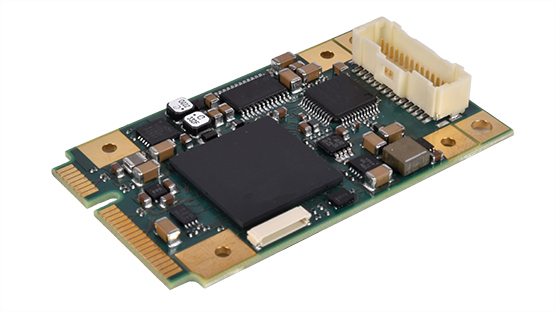
\includegraphics[width=0.7\textwidth]{img/2_steuerung/goat_io397.png}
		\caption{Speedgoat – I/O Module 397 \cite{speedgoat:IO397}}
		\label{img_2_2:goat:IO397}
	\end{center}
\end{figure}

Das IO397 I/O-Modul ist ein mPCIe-kompatibles, in Simulink programmierbares FPGA-Modul mit 50k Logikzellen, 4 ADC-Eingangs- und 4 DAC-Ausgangskanälen, sowie 14 ESD-geschützten TTL-I/O-Leitungen. Es unterstützt eine 16-Bit-Auflösung, softwareseitig auswählbare Spannungen und ist ideal für geschlossene Regelkreise und Hardware-in-the-Loop (HIL)-Simulationen mit MATLAB und Simulink \cite{speedgoat:IO397}.


\begin{figure}[!ht]
	\begin{center}
		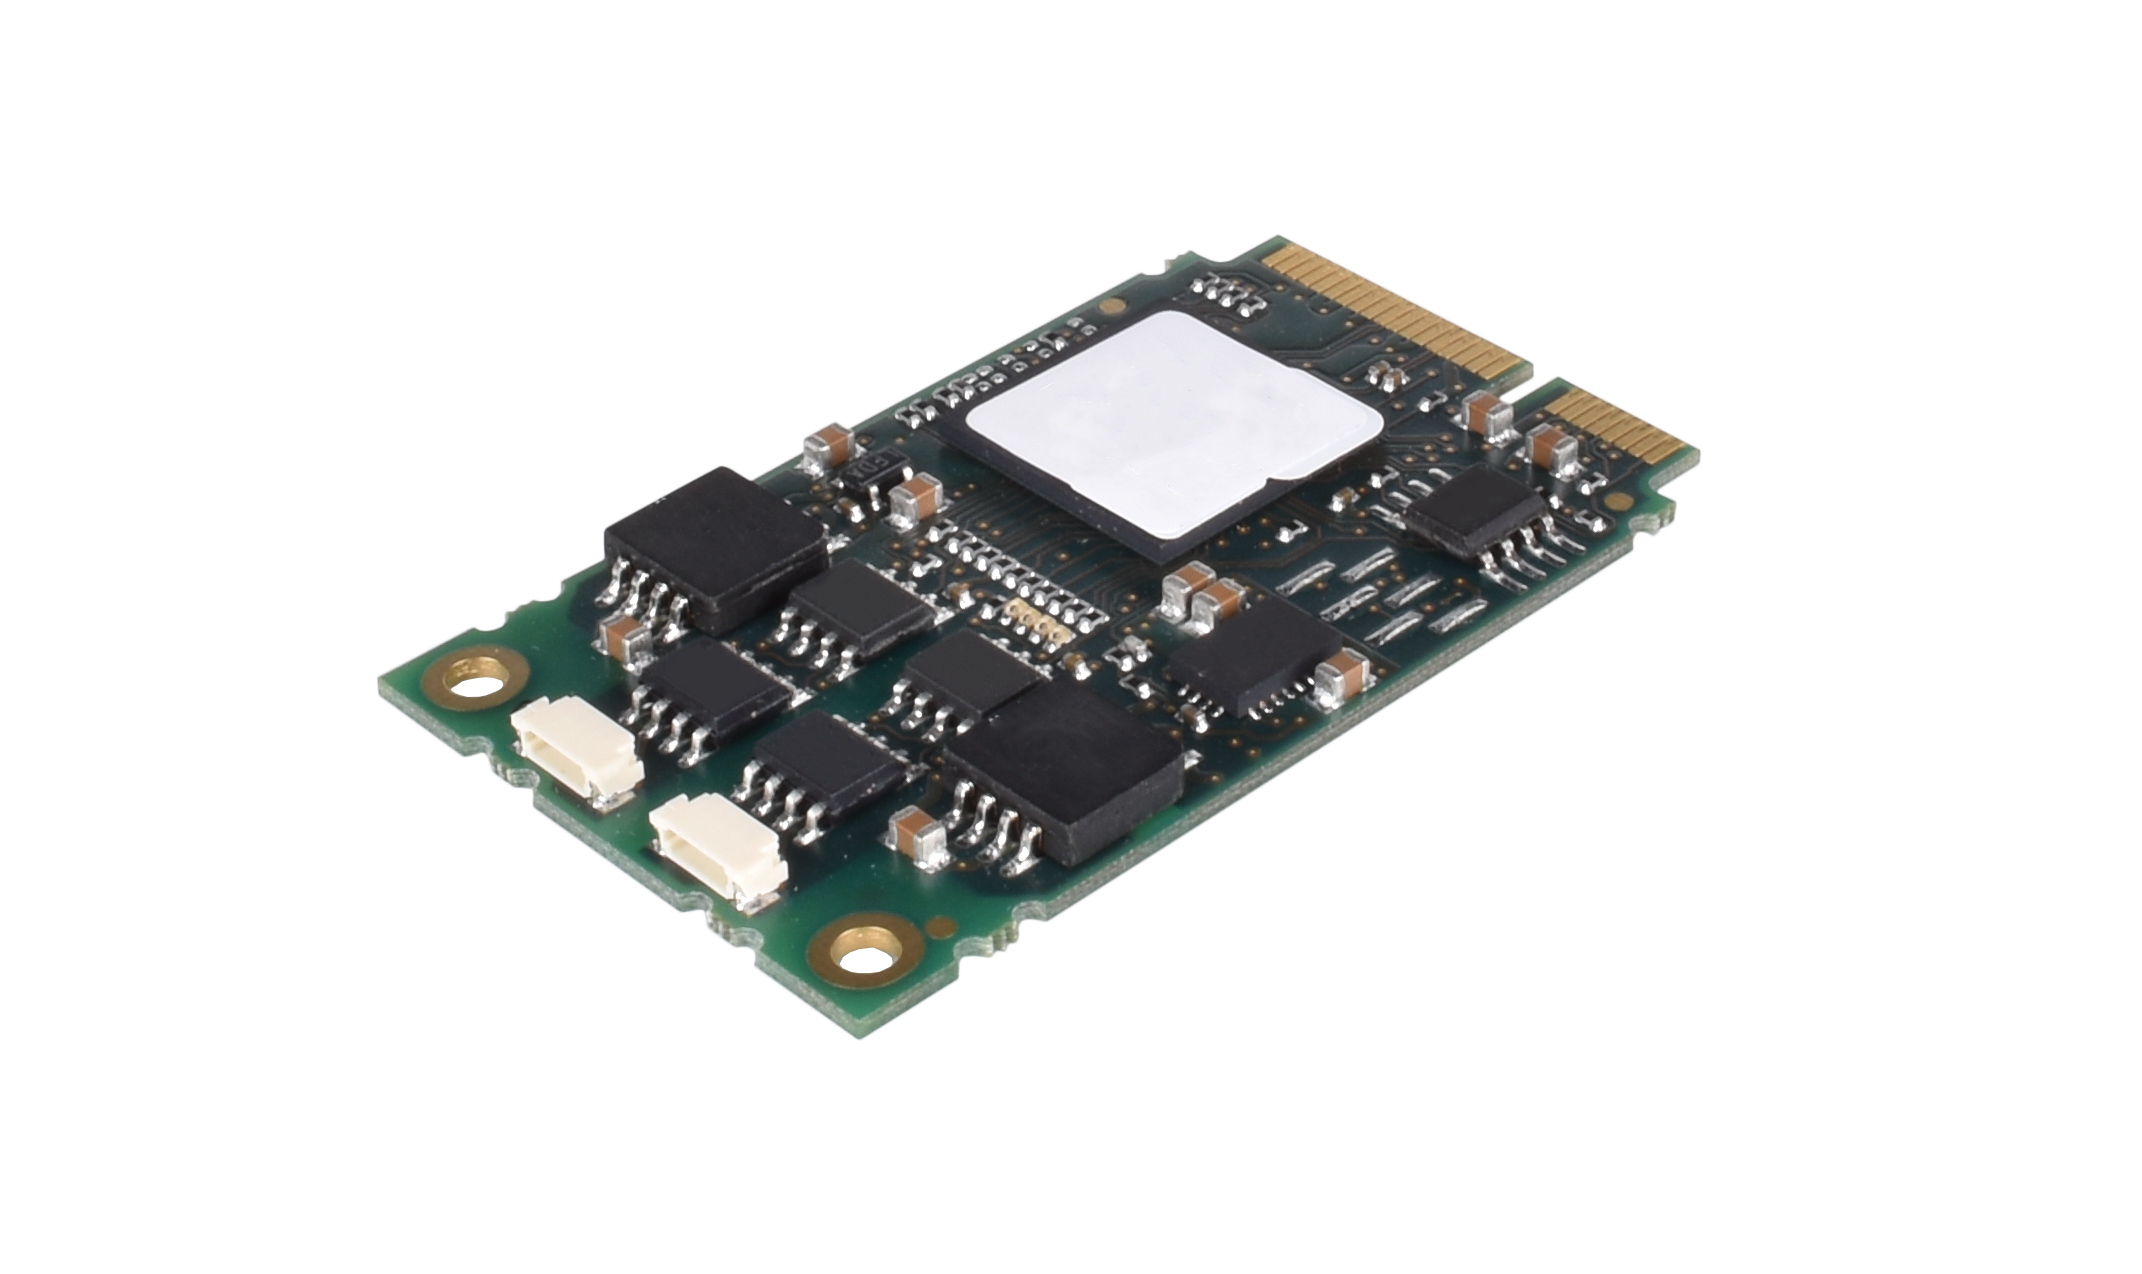
\includegraphics[width=0.7\textwidth]{img/2_steuerung/goat_io691.png}
		\caption{Speedgoat – I/O Module 691 \cite{speedgoat:IO691}}
		\label{img_2_2:goat:IO691}
	\end{center}
\end{figure}

Das IO691 I/O-Modul bietet eine intelligente CAN-Schnittstelle mit zwei Kanälen, die sowohl flexible Datenrate CAN (CAN FD) als auch High-Speed CAN (CAN HS) unterstützen. Es ist kompatibel mit CAN 2.0A/B-Netzwerken und unterstützt SAE J1939 sowie ASAM XCP für Bypassing. Alle Signale sind über 9-polige D-Sub-Front-CAN-Anschlüsse zugänglich. Das Modul ist ideal für geschlossene Regelkreise, Hardware-in-the-Loop-Simulationen und Restbussimulationen mit MATLAB und Simulink \cite{speedgoat:IO691}.

\subsection{Pin Mapping der Module}
Das Modul IO397-50k kann über ein Sensor-Aktor-Kabel von Phoenix Contact extern angeschlossen werden, wie in Abbildung \ref{img_2_2:steuerung_goat:2} dargestellt.
Zusätzlich wird das Modul IO691 mittels eines 9-Pin D-Sub-Steckers (männlich) angeschlossen.

\begin{figure}[!ht]
	\begin{center}
		\includegraphics[width=1\textwidth]{img/2_steuerung/goat_2.png}
		\caption{Speedgoat – Ansicht der Modulanschlüsse}
		\label{img_2_2:steuerung_goat:2}
	\end{center}
\end{figure}

%\begin{figure}[!ht]
%	\begin{center}
%		\includegraphics[width=1\textwidth]{img/2_steuerung/goat_3.png}
%		\caption{Speedgoat – Ansicht der Kommunikationsschnittstellen}
%		\label{img_2_2:steuerung_goat:3}
%	\end{center}
%\end{figure}



\subsubsection{Pin Mapping – IO397-50k}

Terminal Board A ist für die Verarbeitung analoger Signale ausgelegt, sowohl für Eingänge als auch für Ausgänge. Die Tabelle \ref{speedgoat:IO397A} zeigt das Pin Mapping von Terminal Board A. Dieses Board enthält Anschlüsse für insgesamt vier analoge Eingänge (Pins 1a bis 8a) und vier analoge Ausgänge (Pins 9a bis 12a). Die analogen Eingänge sind für die Messung von Spannungen in Bezug auf eine physikalische Große zuständig, wobei die positiven und negativen Leitungen (jeweils '+' und '-') getrennt geführt werden, um eine differenzielle Signalverarbeitung zu ermöglichen. Die Ausgänge sind an einem digitale-zu-analoge-Wandler (DAC) angeschlossen, die analoge Signale für den Antrieb von Geräten bereitstellen. Zusätzlich sind mehrere Ground- und Spannungsanschlüsse vorhanden, um eine stabile Stromversorgung zu gewährleisten.
\pagebreak
\begin{table}[!ht]
	\centering
	\caption{IO397-50k Pin   – Terminal Board A: analog I/O \cite{speedgoat:IO397}}
	\label{speedgoat:IO397A}
	\begin{tabular}{lcl}
		\hline
		\textbf{Pin}             & \textbf{Funktionalität} & \textbf{Type} \\ \hline
		\multicolumn{1}{l|}{1a}  & Analog input 01 (+)     & ADC           \\
		\multicolumn{1}{l|}{2a}  & Analog input 01 (-)     & ADC           \\
		\multicolumn{1}{l|}{3a}  & Analog input 02 (+)     & ADC           \\
		\multicolumn{1}{l|}{4a}  & Analog input 02 (-)     & ADC           \\
		\multicolumn{1}{l|}{5a}  & Analog input 03 (+)     & ADC           \\
		\multicolumn{1}{l|}{6a}  & Analog input 03 (-)     & ADC           \\
		\multicolumn{1}{l|}{7a}  & Analog input 04 (+)     & ADC           \\
		\multicolumn{1}{l|}{8a}  & Analog input 04 (-)     & ADC           \\ \hline
		\multicolumn{1}{l|}{9a}  & Analog output 01        & DAC           \\
		\multicolumn{1}{l|}{10a} & Analog output 02        & DAC           \\
		\multicolumn{1}{l|}{11a} & Analog output 03        & DAC           \\
		\multicolumn{1}{l|}{12a} & Analog output 04        & DAC           \\ \hline
		\multicolumn{1}{l|}{13a} & Ground                  &               \\
		\multicolumn{1}{l|}{14a} & Ground                  &               \\
		\multicolumn{1}{l|}{15a} & 0V                      &               \\
		\multicolumn{1}{l|}{16a} & 5V                      &               \\
		\multicolumn{1}{l|}{17a} & Ground                  &               \\
		\multicolumn{1}{l|}{SH}  & Shielding of M12 cable  &               \\ \hline
	\end{tabular}
\end{table}

Terminal Board B hingegen bietet eine flexible Konfiguration für digitale Ein- und Ausgänge. Die Tabelle \ref{speedgoat:IO397B} zeigt das Pin Mapping von Terminal Board B. Die Pins 3b bis 16b sind für konfigurierbare I/O-Funktionalitäten ausgelegt und nutzen TTL-Signale (Transistor-Transistor-Logik), was sie besonders für schnelle digitale Schaltvorgänge geeignet macht. Dieses Board ermöglicht es, die Anschlüsse flexibel zu nutzen, je nach den Anforderungen der Applikation. Auch hier gibt es mehrere Spannungs- und Ground-Anschlüsse, sowie eine Abschirmung (Shielding) für das M12-Kabel, um elektromagnetische Störungen zu minimieren.
\pagebreak
\begin{table}[!ht]
	\centering
	\caption{IO397-50k Pin Mapping – Terminal Board B: analog I/O \cite{speedgoat:IO397}}
	\label{speedgoat:IO397B}
	\begin{tabular}{lll}
		\hline
		Pin                      & Funktionalität  & Type   \\ \hline
		\multicolumn{1}{l|}{1b}  & 0 V             &        \\
		\multicolumn{1}{l|}{2b}  & 5 V             &        \\ \hline
		\multicolumn{1}{l|}{3b}  & CAP             & IN     \\
		\multicolumn{1}{l|}{4b}  & CAP             & IN     \\
		\multicolumn{1}{l|}{5b}  & CAP             & IN     \\
		\multicolumn{1}{l|}{6b}  & CAP             & IN     \\
		\multicolumn{1}{l|}{7b}  & CAP             & IN     \\
		\multicolumn{1}{l|}{8b}  & CAP             & IN     \\
		\multicolumn{1}{l|}{9b}  & CAP – Trigger   & IN     \\ \hline
		\multicolumn{1}{l|}{10b} & QAE – A         & OUT    \\
		\multicolumn{1}{l|}{11b} & QAE – A         & OUT    \\
		\multicolumn{1}{l|}{12b} & QAE – C/Index   & OUT    \\ \hline
		\multicolumn{1}{l|}{13b} & DIO             & IN/OUT \\
		\multicolumn{1}{l|}{14b} & DIO             & IN/OUT \\
		\multicolumn{1}{l|}{15b} & DIO             & IN/OUT \\
		\multicolumn{1}{l|}{16b} & Interrupt input & IN     \\
		\multicolumn{1}{l|}{17b} & GND             &        \\ \hline
	\end{tabular}
\end{table}



\subsubsection{Pin Mapping –  IO691}


\begin{table}[!ht]
	\centering
	\caption{IO691 Pin Mapping}
	\label{speedgoat:IO691}
	\begin{tabular}{ll}
		\hline
		\textbf{Pin}           & \textbf{DB9 Connector A/B, Signal} \\ \hline
		\multicolumn{1}{l|}{1} & -                                  \\
		\multicolumn{1}{l|}{2} & CAN-low                            \\
		\multicolumn{1}{l|}{3} & GND                                \\
		\multicolumn{1}{l|}{4} & -                                  \\
		\multicolumn{1}{l|}{5} & -                                  \\
		\multicolumn{1}{l|}{6} & GND                                \\
		\multicolumn{1}{l|}{7} & CAN-high                           \\
		\multicolumn{1}{l|}{8} & -                                  \\
		\multicolumn{1}{l|}{9} & -                                  \\ \hline
	\end{tabular}
\end{table}


\section{Abstandsmessung}
\begin{figure}[!ht]
	\begin{center}
		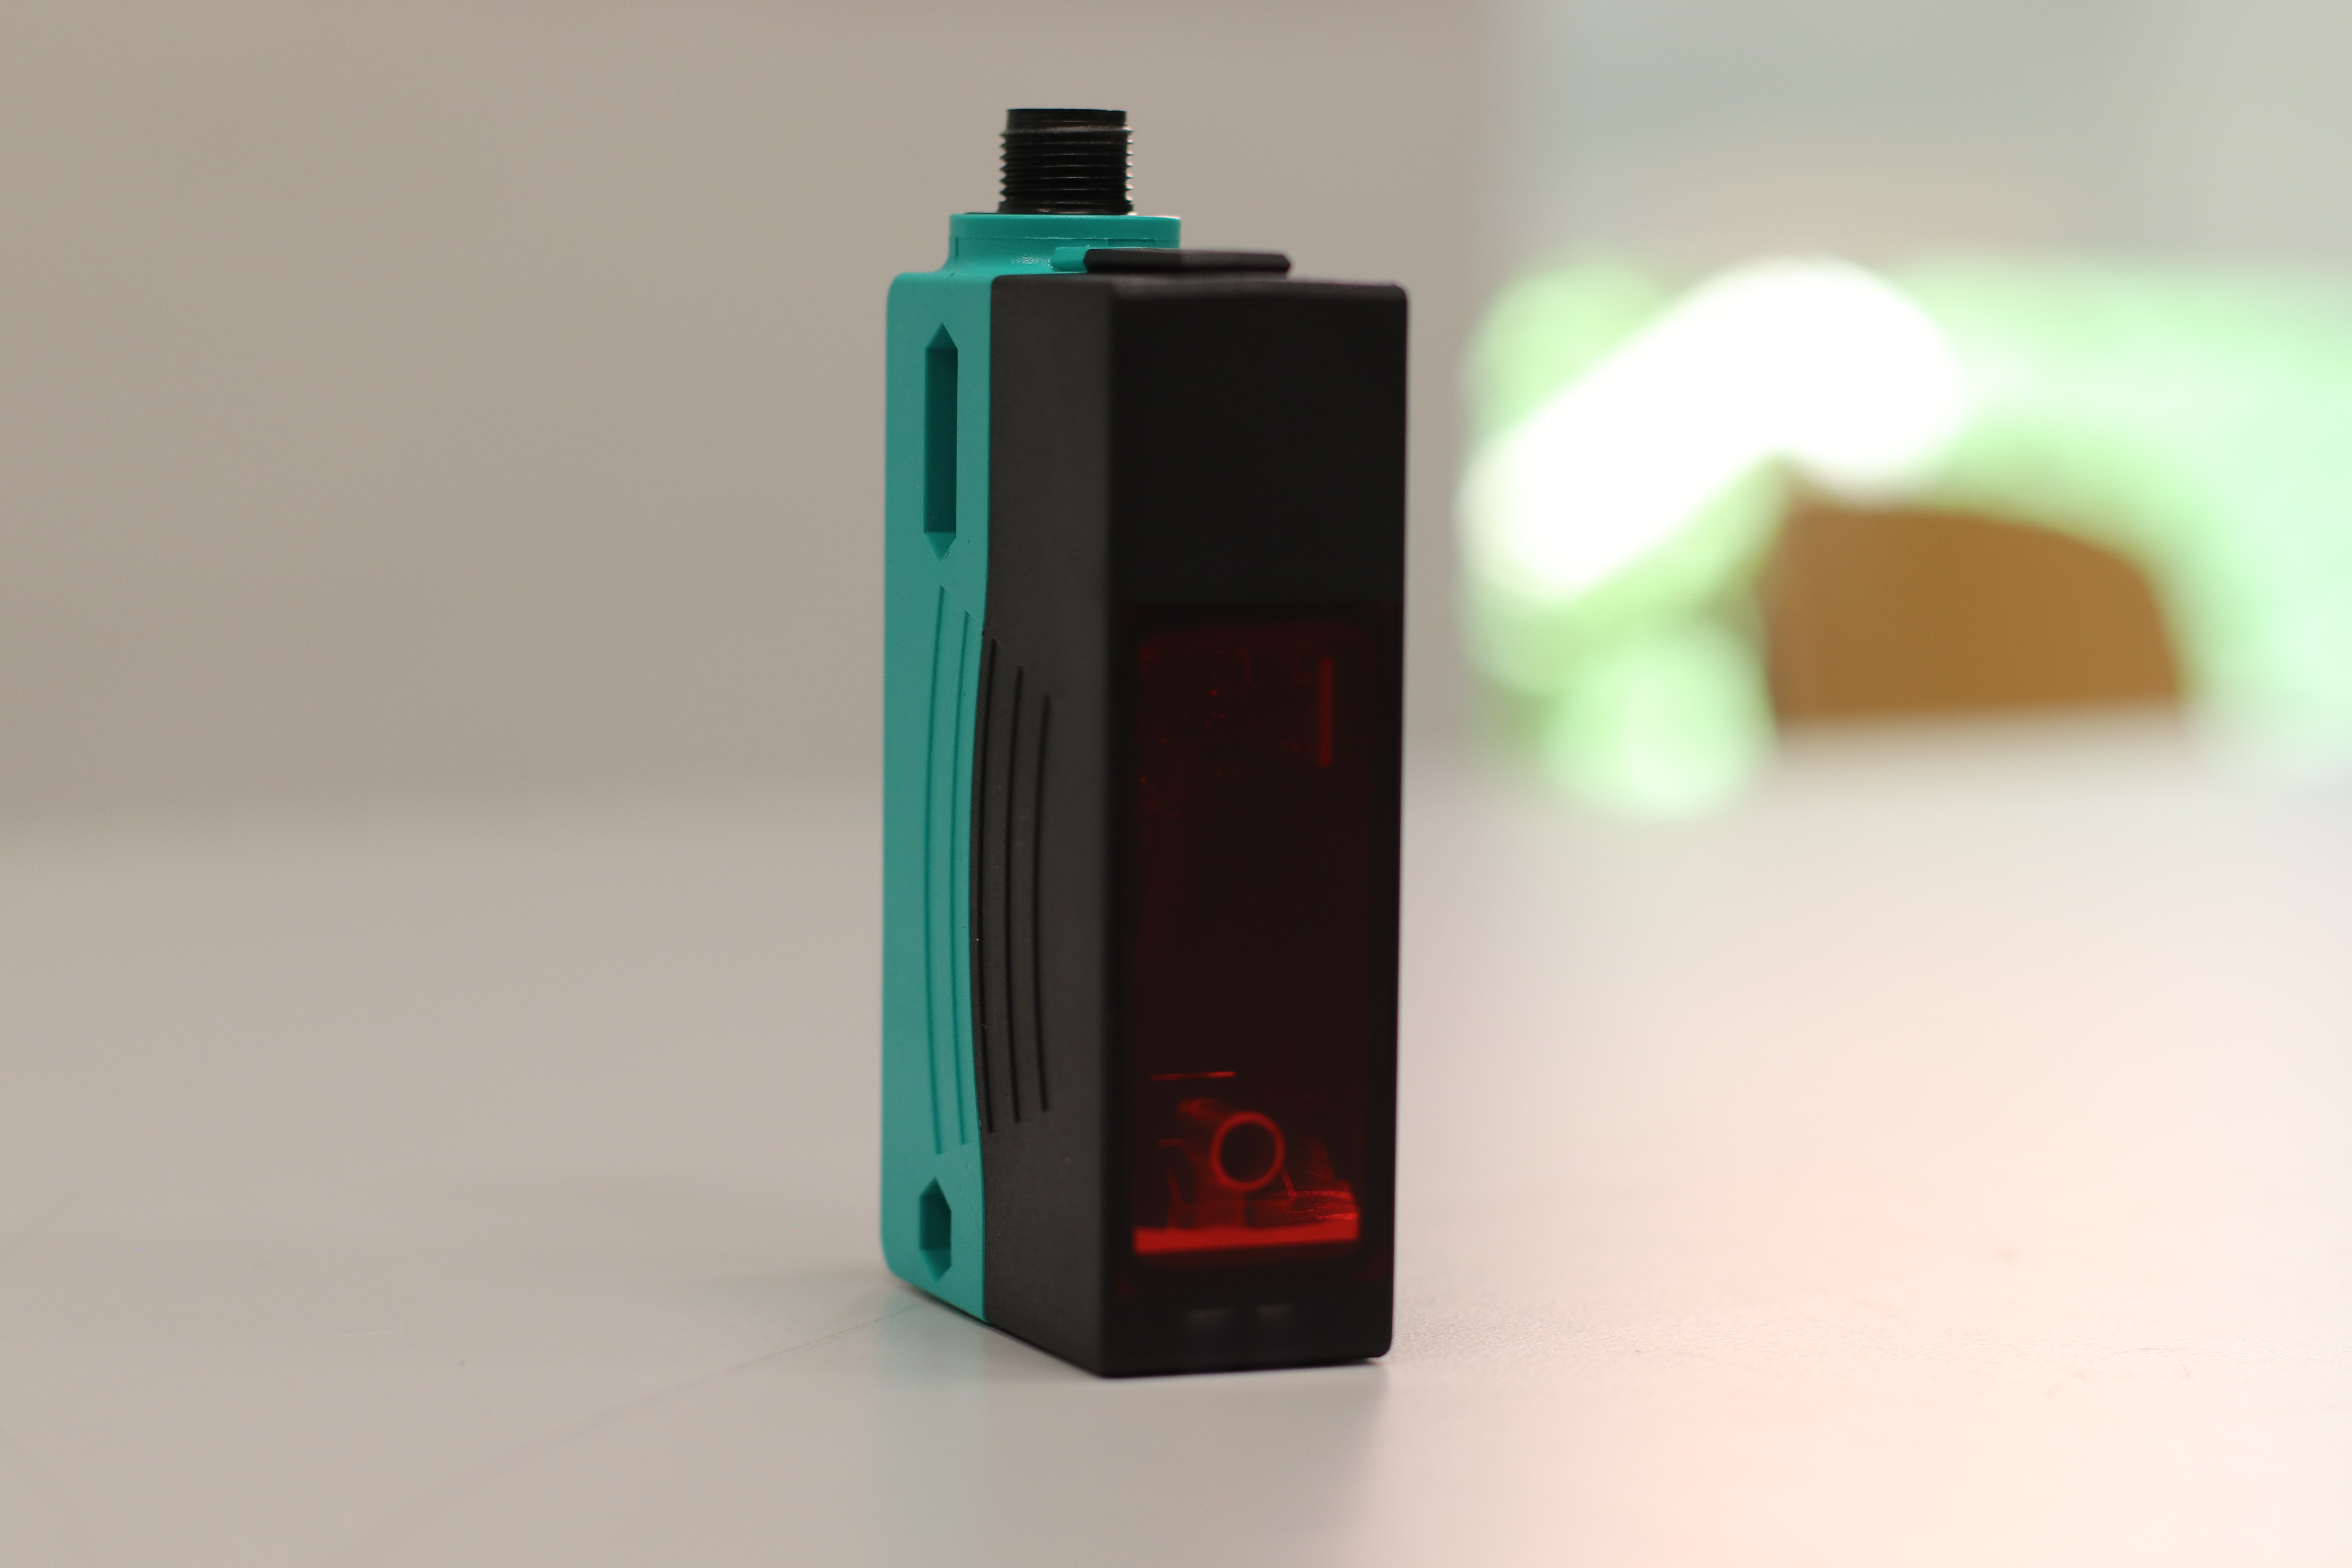
\includegraphics[width=1\textwidth]{img/2_sen/dis_pepperl+fuchs_1.png}
		\caption{Pepperl+Fuchs – Distanzsensor}
		\label{img_2_2:sen_dis:1}
	\end{center}
\end{figure}




\section{Speicher}

\begin{figure}[!ht]
	\begin{center}
		\includegraphics[width=1\textwidth]{img/2_speicher/speicher.png}
		\caption{DeepCPower – Lithium Batterie 50Ah | 51,2V | 2560Wh}
		\label{img_2_2:speicher_1:1}
	\end{center}
\end{figure}


